\chapter{Background} \label{chap:background}

\section{Inverse Problems}\label{sec:inverse-problems}

\begin{definition}[Inverse Problem with Gaussian Noise]\label{def:inverse-problem}
    Given  a data-point $\mathbf{x} \in \mathcal{X} \subseteq \mathbb{R}^{d_x}$,
    denote some lossy measurement by
    \begin{equation}
        \mathbf{y} = m(\mathbf{x}) + \sigma_y\epsilon \in \mathcal{Y},\quad \epsilon \sim \mathcal{N}\left(0, \mathbf{I}_{d_y}\right) \label{eq:inverse-problem}
    \end{equation}
    where $m: \mathcal{X} \to \mathcal{Y} \subseteq \mathbb{R}^{d_y}$ is some \emph{measurement operator},
    and $\sigma_y \in \mathbb{R}^+$ controls the measurement noise. The goal of an inverse problem
    is to recover $\mathbf{x}$ from $\mathbf{y}$. We call $\mathcal{X}$ the \emph{state space} and
    $\mathcal{Y}$ the \emph{measurement space}.
\end{definition}

\begin{definition}[Linear Inverse Problem]\label{def:linear-inverse-problem}
    A linear inverse problem is an inverse problem where the measurement operator is such that
    $h(\mathbf{x}) = A\mathbf{x}$ for some matrix $A \in \mathbb{R}^{d_y \times d_x}$ called the
    \emph{measurement matrix}.
\end{definition}

\begin{example}[Gaussian Deblurring]
    Suppose we have some $\mathbf{x}$ representing a flattened $h\times w$ image (ignoring channels
    for simplicity). Let $h(\mathbf{x})$ represent the convolution of $\mathbf{x}$ with a Gaussian
    kernel. Given the discrete nature of images, this kernel can be represented as a
    $k \times k$ matrix. Given that the convolution operator is linear, we can form some matrix $A$
    from the kernel matrix (by using it to form a block Toeplitz matrix) so that
    $h(\mathbf{x}) = A\mathbf{x}$. It follows that if we have some blurry image, $\mathbf{y}$,
    generated according to \autoref{eq:inverse-problem}, the goal of inferring the unblurred image,
    $\mathbf{x}$, represents a linear inverse problem.
\end{example}

\begin{figure}[htbp]
    \centering
    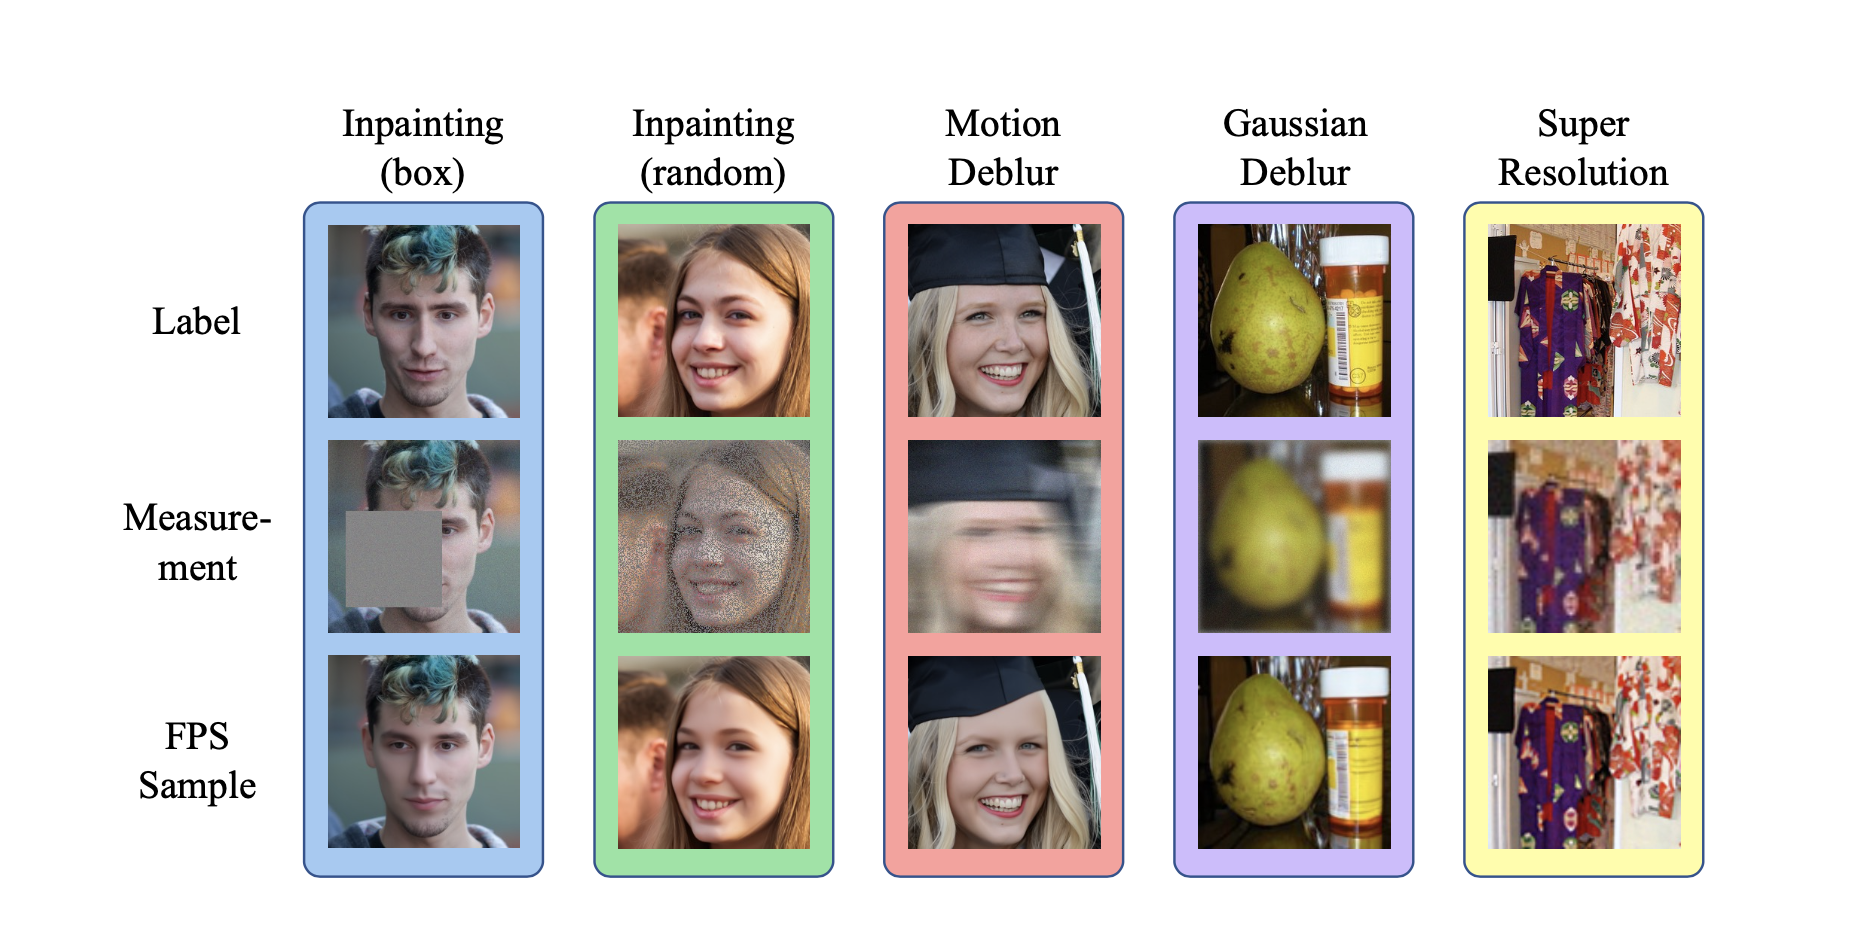
\includegraphics[width=1\textwidth]{assets/inverse_problems.png}
    \caption{Examples of inverse problems for image data \parencite{douDiffusionPosteriorSampling2023}.}
    \label{fig:inverse-problems}
\end{figure}

\begin{remark}[Bayesian Solution to Ill-posed Inverse Problems] \label{rem:bayes-inv}
    Typically $d_x > d_y$, leading to a many-to-one $\mathbf{x} \rightarrow \mathbf{y}$ mapping
    \parencite{chungDiffusionPosteriorSampling2022}, and requiring some \emph{prior} information
    about $\mathbf{x}$. We call such an inverse problem \emph{ill-posed}. If we assume some prior
    distribution of the data, $p(\mathbf{x})$, ``solving'' the inverse problem amounts to sampling
    from some posterior:
    \begin{equation*}
        p(\mathbf{x} \mid \mathbf{y}) \propto p(\mathbf{x})g(\mathbf{y} \mid \mathbf{x})
        = p(\mathbf{x})\mathcal{N}\left(\mathbf{y} \mid m(\mathbf{x}), \sigma^2_y\mathbf{I}_{d_y}\right)
    \end{equation*}
    For many problems, $p(\mathbf{x})$ is generally unknown or does not conjugate with
    $g(\mathbf{y} \mid \mathbf{x})$, necessitating numerical methods to sample from
    $p(\mathbf{x} \mid \mathbf{y})$.
\end{remark}

\section{General Optimisation through Sampling}\label{sec:general-optimisation}

\begin{definition}[Gibbs Measure / Boltzmann Distribution]
    Let $\mathcal{X} \subseteq \mathbb{R}^{d_x}$ be a state space and let
    $h: \mathcal{X} \rightarrow \mathbb{R}$ be a measurable function, called the
    \emph{energy function} or \emph{Hamiltonian}. The Gibbs measure is the probability density
    function over $\mathcal{X}$ given by:
    \begin{equation}
        q(\mathbf{x}; \beta) = \frac{\exp\{-\beta h(\mathbf{x})\}}{Z(\beta)} \label{eq:gibbs-measure}
    \end{equation}
    where $\beta > 0$ is the \emph{inverse temperature} parameter and $Z(\beta)$ is the normalizing
    constant (also known as the partition function), defined by:
    \begin{equation*}
        Z(\beta) = \int_{\mathcal{X}} \exp\{-\beta h(\mathbf{x})\} \, d\mathbf{x}
    \end{equation*}
\end{definition}

\begin{proposition}[Optimization via Sampling
    \parencite{hwangLaplaceMethodRevisited1980, kongDiffusionModelsConstrained2024}] \label{prop:opt-sampling}
    Assume $h \in \mathrm{C}^3(\mathbb{R}^{d_x}, \mathbb{R})$ with $\{\mathbf{x}_i^*\}_{i=1}^M$ the
    set of its minimizers. Let $p$ be a density on $\mathbb{R}^d$ such that there exists
    $i_0 \in \{1, \dots, M\}$ with $p(\mathbf{x}_{i_0}^*) > 0$. Then $Q_\beta$, the distribution
    with density w.r.t the Lebesgue measure $\propto q(\mathbf{x}; \beta)p(\mathbf{x})$, weakly
    converges to $Q_{\infty}$ as $\beta \rightarrow \infty$ and we have that:
    \begin{equation}
        Q_\infty = \frac{\sum_{i=1}^{M}a_i\delta_{\mathbf{x}_i^*}}{\sum_{i=1}^{M}a_i} \label{eq:opt-target-inf}
    \end{equation}
    with $a_i = p(\mathbf{x}_i^*)\det(\nabla^2h(\mathbf{x}_i^*))^{-1/2}$
\end{proposition}

\begin{remark}[Annealing]
    \autoref{prop:opt-sampling} tells us that by properly \emph{tempering}
    $\beta$ (i.e. slowly increasing it), we can globally optimize (minimize or maximize via
    negation) the function $h$. Note here that because $\beta$ is the \emph{inverse} temperature,
    we refer to increasing it as \emph{annealing} (lowering the temperature). The density function
    $p$ can be interpreted as some \emph{prior} distribution we use to sample the points $\mathbf{x}$
    (ideally such that more `mass' is placed near the optima, $\{\mathbf{x}_i^*\}_{i=1}^M$,
    \emph{a priori}).
\end{remark}

\section{Diffusion Models}\label{sec:diffusion-models}

\begin{definition}[Stein Score] \label{def:stein-score}
    Given a probability density function $p(\mathbf{x})$ on $\mathbb{R}^{d_x}$, the Stein score
    function is given by $\nabla_{\mathbf{x}} \log p(\mathbf{x})$, the gradient of the log-density
    with respect to the data (\emph{not} the distribution's parameters).
    Going forwards, we refer to the Stein score simply as the \emph{score}, in-line with convention in
    related literature.
\end{definition}

\begin{definition}[Forwards Noising Process \parencite{douDiffusionPosteriorSampling2023}] \label{def:forward-process}
    Let $\mathbf{x}_0$ be a sample from some $p_{\text{data}}$ distribution. Define the
    \emph{forward noising process} as a Markov chain:
    \begin{equation*}
    q(\mathbf{x}_{1:T} \mid \mathbf{x}_0) = \prod_{t=1}^T \mathcal{N}\left(a_t \mathbf{x}_{t-1}, b_t^2\mathrm{I}_{d_x}\right) \label{eq:fwd}
    \end{equation*}
    where $\{(a_t, b_t)\}_{t=1}^T$ differ depending on formulation of the problem, and $T$ is
    typically quite large ($\approx 1000$). $a_t$ and $b_t$ can be interpreted as the
    \emph{memory retention factor} and \emph{noise magnitude} of the forward process which typically
    decrease and increase, respectively, with time.
\end{definition}

\begin{definition}[Forward Marginal \parencite{douDiffusionPosteriorSampling2023}]
    Given some forward noising process defined by $\{(a_t, b_t)\}_{t=1}^T$, the
    \emph{forward marginal} is given by:
    $$
    q(\mathbf{x}_t \mid \mathbf{x}_0) = \mathcal{N}(c_t\mathbf{x}_0, d_t^2\mathrm{I}_{d_x})
    $$
    where $c_t, d_t$ are derived from $a_t$ and $b_t$. $c_t$ essentially represents the signal
    strength (from the original sample) while $d_t$ represents the cumulative noise. It follows that
    we should have $c_T \approx 0, d_T \approx 1$ since the goal is to fully destructure the data
    into $\mathcal{N}(0, \mathbf{I}_{d_x})$ noise.
\end{definition}

\begin{definition}[Backwards Denoising Process \parencite{douDiffusionPosteriorSampling2023}] \label{def:backwards-process}
    Given some forward noising process, we assume\footnote{This assumption is well-founded for
    large $T$ since the forward processes associated SDE (see \autoref{rem:sde-rep}) can be
    analytically reversed using the score thanks to the result of
    \textcite{andersonReversetimeDiffusionEquation1982}. This, along with reducing the
    discretisation error of sampling from the SDE, is why we take $T$ as large as feasible.
    \label{ftnt:sde-rep}} some backwards process ($t=T \to 0$) to be likewise a Markov chain with
    one-step backwards transition kernel given by:
    \begin{equation}
        p(\mathbf{x}_{t-1} \mid \mathbf{x}_t) = \mathcal{N}\left(u_t\cdot \hat{\mathbf{x}}_0(\mathbf{x}_t) + v_t\nabla_{\mathbf{x}_t}\log q(\mathbf{x}_t), w_t^2\mathrm{I}_{d_x}\right) \label{eq:backwards-process}
    \end{equation}
    with $u_t, v_t$ some functions of $a_t, b_t$,
    $q(\mathbf{x}_t) = \int q(\mathbf{x}_t \mid \mathbf{x}_0)p(\mathbf{x}_0)\, d\mathbf{x}_0$, and:
    \begin{equation}
        \hat{\mathbf{x}}_0(\mathbf{x}_t) := \EE{\mathbf{x}_0 \mid \mathbf{x}_t} = \frac{\mathbf{x}_t + d_t^2\nabla_{\mathbf{x}_t}\log q(\mathbf{x}_t)}{c_t} \label{eq:tweedie}
    \end{equation}
    derived from Tweedie's formula.
\end{definition}

\begin{remark}[DDPM Representation]
    Under the de-noising diffusion probabilistic model (DDPM) of
    \textcite{hoDenoisingDiffusionProbabilistic2020}, we take:
    \begin{equation}
        a_t = \sqrt{\alpha_t} \quad
        b_t = \sqrt{\beta_t} \quad
        c_t = \sqrt{\overline{\alpha}_t} \quad
        d_t = \sqrt{1 - \overline{\alpha}_t}
    \end{equation}
    and
    \begin{equation}
        u_t = \sqrt{\overline{\alpha}_{t-1}}\footnote{In \textcite{douDiffusionPosteriorSampling2023} this is incorrectly given as $\sqrt{\alpha_{t-1}}$.} \quad
        v_t = -\sqrt{\alpha_t}(1 - \overline{\alpha}_{t-1}) \quad
        w_t = \sqrt{\beta_t \cdot \frac{1 - \overline{\alpha}_{t-1}}{1 - \overline{\alpha}_t}}
    \end{equation}
    with $\alpha_t = 1 - \beta_t$, for some $\beta_t \in (0, 1)$ known as the \emph{noise schedule},
    and $\overline{\alpha}_t = \prod_{\tau=1}^{t}\alpha_\tau$.
    For this paper, we primarily consider the DDPM formulation for simplicity. However, other
    formulations, such as de-noising diffusion implicit models (DDIM) of
    \textcite{songDenoisingDiffusionImplicit2020} (see \autoref{rem:ddim}) and Predictor-Corrector (PC)
    \textcite{songScoreBasedGenerativeModeling2021}, are equally applicable to our proposed framework;
    the only requirement is that the formulations conform to the above representations of the forwards
    and backwards process, and enable sampling at discrete time points.
\end{remark}

\begin{remark}[Noise Schedule]
    Under the DDPM framework, the core parameter to tune is the noising schedule, $\beta_t$.
    Typically, we take this as an increasing function from some very low $\beta_{\text{min}}$ to
    some $\beta_{\text{max}}$. A linear schedule is the obvious and common choice, but other
    schedules, such as the cosine schedule of \textcite{nicholImprovedDenoisingDiffusion2021}, can
    lead to better sampling performance. For this paper, the exact details of the schedule are not
    of significant importance; for experiments we use the linear schedule.
\end{remark}

\begin{proposition}[Score to Noise Conversion] \label{prop:score-to-noise}
    Let $\mathbf{x}_t = c_t\mathbf{x}_0 + d_t\epsilon_t$ be a forward noised observation. Then
    $$
    \nabla_{\mathbf{x}_t} \log q_t(\mathbf{x}_t) \approx -\frac{\mathbf{\epsilon}_t}{d_t}.
    $$
\end{proposition}
\begin{proof}
    Follows from forward marginal and Tweedie's formula (\autoref{eq:tweedie}).
\end{proof}

Given \autoref{def:backwards-process} (and \autoref{prop:score-to-noise}), it follows that if we have
access to the score (or noise added), we can sample from $p_{\text{data}}$ by sampling
$\mathbf{x}_T \sim \mathcal{N}(0, \mathbf{I}_{d_x})$ ($\approx q(\mathbf{x}_T \mid \mathbf{x}_0)$)
and iterating backwards in time according to \autoref{eq:backwards-process} until $t=0$.

Unfortunately, $\nabla_{\mathbf{x}_t}\log q(\mathbf{x}_t)$ is intractable\footnote{Note this is not
$\nabla_{\mathbf{x}_t}\log q(\mathbf{x}_t \mid \mathbf{x}_0)$, which is tractable but ``useless''
for sampling since we don't know $\mathbf{x}_0$ a priori (it's what we're trying to sample); this
quantity is useful, however, for training where we \emph{do} know $\mathbf{x}_0$.}.
As such, we train a score-approximating \parencite{songScoreBasedGenerativeModeling2021} (or
noise-predicting \parencite{hoDenoisingDiffusionProbabilistic2020}, and apply
\autoref{prop:score-to-noise}) neural network, denoted $s_\theta(\mathbf{x}_t, t)$
($\epsilon_\theta(\mathbf{x}_t, t)$). We defer to the extensive literature (foundationally
\textcite{hoDenoisingDiffusionProbabilistic2020}, \textcite{songGenerativeModelingEstimating2020},
\textcite{songScoreBasedGenerativeModeling2021} and \textcite{nicholImprovedDenoisingDiffusion2021})
on how precisely to train such a network, but generally this is achieved via minimization of a
``re-weighted variant of the evidence lower bound''
\parencite{songScoreBasedGenerativeModeling2021}; e.g. for a score network:
\begin{equation*}
    \theta^* = \underset{\theta}{\arg\min}\sum_{t=1}^T (1 - \alpha_t)\mathbb{E}_{\mathbf{x}_0 \sim \hat{p}_{\text{data}}}\mathbb{E}_{\mathbf{x}_t \mid \mathbf{x}_0 \sim q_{\alpha_t}}\left[\Vert s_\theta(\mathbf{x}_t, t) - \nabla_{\mathbf{x}_t}\log q_{\alpha_t}(\mathbf{x}_t \mid \mathbf{x}_0)\Vert_2^2\right]
\end{equation*}

where $\hat{p}_{\text{data}}$ is the empirical data distribution (i.e. based on our training
samples), and $q_{\alpha_t}$ is the forward marginal at time $t$.

Plugging in this score network to \autoref{eq:backwards-process}, we yield an approximate
\emph{backwards transition kernel},
$p_\theta(\mathbf{x}_{t-1} \mid \mathbf{x}_t) \approx q(\mathbf{x}_{t-1} \mid x_t)$, which we use to
sample backwards in time. Formally, we sample according to:
\begin{equation}
    p_\theta(\mathbf{x}_0) = \int p(\mathbf{x}_T)\prod_{t=1}^T p_\theta(\mathbf{x}_{t-1} \mid \mathbf{x}_{t})\, d\mathbf{x}_{1:T},\quad p(\mathbf{x}_T) = \mathcal{N}(\mathbf{x}_T; 0, \mathbf{I}_{d_x}) \label{eq:uncond-sampling}
\end{equation}
with, given a well trained network, $p_\theta(\mathbf{x}_0) \approx p_{\text{data}}(\mathbf{x}_0)$.
Denote the mean of this transition kernel by $\mu_t(\mathbf{x}_t, \theta)$ and the variance by
$\Sigma_t$. For DDPM, we have:
\begin{align}
    \mu_t(\mathbf{x}_t, \theta) &= \frac{1}{\sqrt{\alpha_t}}\mathbf{x}_{t} + \frac{\beta_t}{\sqrt{\alpha_t}}s_\theta(\mathbf{x}_t, t) \label{eq:ddpm-mu} \\
    \Sigma_t &= \frac{\beta_t(1 - \overline{\alpha}_{t-1})}{1 - \overline{\alpha}_t}\cdot \mathbf{I} \label{eq:ddpm-sigma}
\end{align}

\section{Sequential Monte Carlo}

\begin{definition}[State Space Model] \label{def:ssm}
    Let $\mathbf{x}_t \in \mathcal{X}$ be a \emph{state vector} at time $t$, which encapsulates all
    the information about some system necessary to predict future states (perhaps stochastically).
    Let $\mathbf{y}_t \in \mathcal{Y}$ be some observation vector at time $t$, representing
    (potentially noisy) measurements of the system. Let $\phi: \mathcal{X} \to \mathcal{X}$ be some
    function we call the \emph{transition function}. Let $m: \mathcal{X} \to \mathcal{Y}$ be a
    measurement operator. Then the following dynamical system represents a (Gaussian)
    \emph{state space model} (SSM):
    \begin{align}
        \mathbf{X}_t \mid \mathbf{X}_{t-1} = \mathbf{x}_{t-1} &\sim \mathcal{N}(\phi(\mathbf{x}_{t-1}), \sigma_x^2 \mathbf{I}_{d_x}) \label{eq:ssm-proposal} \\
        \mathbf{Y}_t \mid \mathbf{X_t} = \mathbf{x}_t &\sim \mathcal{N}(m(\mathbf{x}_t), \sigma_y^2 \mathbf{I}_{d_y}) \label{eq:ssm-likelihood}
    \end{align}
    We refer to \autoref{eq:ssm-proposal} as the \emph{transition kernel}, with density
    $f(\mathbf{x}_t \mid \mathbf{x}_{t-1})$, and \autoref{eq:ssm-likelihood} as the \emph{likelihood},
    with density $g(\mathbf{y}_t \mid \mathbf{x}_t)$.
\end{definition}

\begin{definition}[Bayesian Filtering] \label{def:bayesian-filtering}
    Suppose we have access to measurements $\mathbf{y}_{0:t}$ emitted from some
    SSM. The task of using such measurements to infer the hidden states, $\mathbf{x}_{0:t}$, is
    known as \emph{Bayesian filtering}. We may be interested in the
    \emph{joint filtering distribution}, with density $p(\mathbf{x}_{0:t} \mid \mathbf{y}_{0:t})$,
    or the \emph{filtering distribution}, with density $p(\mathbf{x}_t \mid \mathbf{y}_{0:t})$.
    Focusing on the latter, given the setup of \autoref{def:ssm}, we can derive the two-step recursive
    relationship:
    \begin{align}
        p(\mathbf{x}_t \mid \mathbf{y}_{0:t-1}) &= \int p(\mathbf{x}_t, \mathbf{x}_{t-1} \mid \mathbf{y}_{0:t-1})\, d\mathbf{x}_{t-1} \nonumber \\
        &= \int f(\mathbf{x}_t \mid \mathbf{x}_{t - 1})p(\mathbf{x}_{t-1} \mid \mathbf{y}_{0:t-1})\, d\mathbf{x}_{t-1} \label{eq:bayesian-filtering-1} \\
        p(\mathbf{x}_t \mid \mathbf{y}_{0:t}) &\propto p(\mathbf{x}_t, \mathbf{y}_t \mid \mathbf{y}_{0:t-1}) \nonumber \\
        &\propto p(\mathbf{x}_t \mid \mathbf{y}_{0:t-1})g(\mathbf{y}_t \mid \mathbf{x}_t) \label{eq:bayesian-filtering-2}
    \end{align}
    Generally, however, the integral in \autoref{eq:bayesian-filtering-1} and normalising constant in
    \autoref{eq:bayesian-filtering-2} are intractable, necessitating approximate methods.
\end{definition}

\begin{definition}[Sequential Monte Carlo for Filtering\footnote{Also known as Particle Filtering.}] \label{def:smc}
    Sequential Monte Carlo (SMC) provides a method for approximately sampling from the sequence of
    distributions as described in \autoref{def:bayesian-filtering}
    \parencite{chopinIntroductionSequentialMonte2020}. It works by generating $N$ particles,
    $\{\mathbf{x}_t^{(i)}\}_{i=1}^N$, according to some initial distribution, $r_0(\cdot)$,
    moving them according to some \emph{proposal distribution},
    $r_t(\cdot \mid \mathbf{x}_{t-1}, \mathbf{y}_{t})$, weighting the particles according to
    some weighting function, $\omega_t(\mathbf{x}_t, \mathbf{x}_{t-1}, \mathbf{y}_t)$, and
    resampling\footnote{We present multinomial resampling for simplicity, but in practice
    alternative methods, such as systematic resampling, are used due to inefficiencies in the
    multinomial scheme \parencite{chopinIntroductionSequentialMonte2020}} the particles according to
    their (self-normalised) weights ($W_t^{(i)}$). That is, the algorithm takes the following steps
    from $t=1,\ldots,T$:
    \begin{itemize}
        \item \textbf{Propose}: $\tilde{\mathbf{x}}_t^{(i)} \sim r_t(\cdot \mid \mathbf{x}_{t-1}^{(i)}, \mathbf{y}_t), \quad i = 1,\ldots,N$
        \item \textbf{Weight}: $W_t^{(i)} \leftarrowtail \omega_t^{(i)} \leftarrow \omega_t(\tilde{\mathbf{x}}_t^{(i)}, \mathbf{x}_{t-1}^{(i)}, \mathbf{y}_t) \quad i = 1,\ldots,N$
        \item \textbf{Resample}: $\{\mathbf{x}_{0:t}^{(i)}\}_{i=1}^N \sim \text{Multinomial}\left(\{\tilde{\mathbf{x}}_{0:t}^{(i)}\}_{i=1}^N; \{W^{(i)}\}_{i=1}^N\right)$
    \end{itemize}
    At the last step, we can yield an empirical distribution over the particles:
    \begin{equation*}
        \hat{p}(\mathbf{x}_T \mid \mathbf{y}_{0:T}) = \sum_{i=1}^N W_{T}^{(i)}\delta_{\mathbf{x}_{T}^{(i)}(\mathbf{x}_T)}
    \end{equation*}
    which asymptotically (in $N$) approximates the true posterior distribution,
    $p(\mathbf{x}_T \mid \mathbf{y}_{0:T})$ \parencite{delmoralCentralLimitTheorems2011,chopinIntroductionSequentialMonte2020}.
\end{definition}

\begin{remark}[Weight Function]
    The weight function's purpose is to correct for discrepancies between the proposal and true
    posterior, $p(\mathbf{x}_t \mid \mathbf{x}_{t-1}, \mathbf{y}_t)$, which it aims to approximate. In the
    filtering case for an SSM as in \autoref{def:ssm}, the weight function is given by the ratio of the
    two \parencite{chopinIntroductionSequentialMonte2020}:
    \begin{equation}
        \omega_t^{(i)} = \frac{p(\tilde{\mathbf{x}}_t^{(i)} \mid \mathbf{x}_{t-1}^{(i)}, \mathbf{y}_t)}{r_t(\tilde{\mathbf{x}}_t^{(i)} \mid \mathbf{x}_{t-1}^{(i)}, \mathbf{y}_{t})}
        \propto \frac{f(\tilde{\mathbf{x}}_t \mid \mathbf{x}_{t-1}^{(i)})g(\mathbf{y}_t \mid \tilde{\mathbf{x}}_t^{(i)})}{r_t(\mathbf{x}_t \mid \mathbf{x}_{t-1}, \mathbf{y}_{t})} \label{eq:weight-func-gen}
    \end{equation}
\end{remark}

\begin{remark}[Resampling]
    The purpose of resampling is to avoid the issue of weight-degeneracy. Without resampling,
    after several iterations (i.e. for large $T$), most particles will end up having negligible
    weight (since without resampling we need to multiply all previous weights for the particle to
    get its time $t$ weight) and eventually a single particle will dominate the approximation.
    Without resampling, we would not get the desired asymptotic results.
\end{remark}

\section{Related Work} \label{sec:related-work}

The goal of conditionally sampling from $p_{\text{data}}$ (learnt via a diffusion model) based on
some $\mathbf{y}$ has been the center of significant recent research. The principle approach of most
methods is to approximate $\nabla_{\mathbf{x}_t}\log q(\mathbf{x}_t \mid \mathbf{y})$, and plug this
in to \autoref{eq:backwards-process} in place of its unconditional counterpart. The obvious approach is
to train a conditional model to learn some $s_{\theta}(\mathbf{x}_t, \mathbf{y}, t)$ and use this.
Indeed, this is the approach that modern text-to-image, image-to-image, and image-to-video
applications take \parencite{nicholGLIDEPhotorealisticImage2021,liDiffusionModelsImage2023,
sahariaPaletteImagetoImageDiffusion2021,sahariaPaletteImagetoImageDiffusion2021,
rombachHighResolutionImageSynthesis2021}. This approach generally achieves the best conditional
sampling but is limited in application; it requires training a model specific to each particular
inverse problem (of which the aforementioned are examples) which may be costly. Furthermore, such
training requires having labelled data which may impose limitations in certain settings and for
certain tasks.

A separate branch of research, and the area with which this work aligns, considers taking a pre-trained
\emph{unconditional} diffusion model (i.e. one where we just have a parametrised estimator of
$\nabla_{\mathbf{x}_t}\log q(\mathbf{x}_t)$) and \emph{guide} the diffusion process to enable
conditional sampling. This is typically achieved by exploiting the following relationship:
\begin{equation}
    \nabla_{\mathbf{x}_t} \log p_t(\mathbf{x}_t \mid \mathbf{y}) = \nabla_{\mathbf{x}_t} \log p_t(\mathbf{x}_t) + \nabla_{\mathbf{x}_t}\log p_t(\mathbf{y} \mid \mathbf{x}_t) \label{eq:cond-score}
\end{equation}
Replacing the first term with our pre-trained score network, optimal guidance can be achieved then
by well-approximating $\nabla_{\mathbf{x}_t}\log p_t(\mathbf{y} \mid \mathbf{x}_t)$ (which is
intractable). Such approximation methods are generally non-specific to the inverse problem, enabling
taking any unconditional diffusion model and using it to sample from the desired posterior
distribution. The diffusion-posterior-sampling method of
\textcite{chungDiffusionPosteriorSampling2022} was foundational, and can be applied to solve general
inverse problems. \textcite{song2023pseudoinverseguided} and, recently,
\textcite{boysTweedieMomentProjected2023} have iterated on this with more analytically
refined\footnote{See \cite{boysTweedieMomentProjected2023} Section 5 for an excellent summary
of how the methods co-relate.}
approaches (though these are only applicable to linear inverse problems).

Given the difficulty of such approximations, and the sequential nature of the sampling procedure
from diffusion models, significant recent research
\parencite{cardosoMonteCarloGuided2023,trippeDiffusionProbabilisticModeling2023,
wuPracticalAsymptoticallyExact2023,douDiffusionPosteriorSampling2023,
janatiDivideandConquerPosteriorSampling2024} has considered using SMC methods (with time running
from $t=T \to 0$) to instead more directly target the posterior (or rather, the intermediate
distributions $p(\mathbf{x}_t \mid \mathbf{y})$) and circumvent the need to compute this term. Our
framework is most heavily inspired by the scheme of \textcite{cardosoMonteCarloGuided2023}; in
\autoref{sec:relation-to-related} we demonstrate how their scheme is very closely related to our
framework. In fact, each of these methods can be applied under our framework since their differences
essentially lie primarily in their choice of proposal distribution.

However, our framework is generalised to solving any optimization task (not just inverse problems).
Through this lens, our framework's objective and formulation aligns with that of
\cite{kongDiffusionModelsConstrained2024}, with both employing \autoref{prop:opt-sampling} and
essentially targeting the distribution induced by the diffusion model and the objective's
associated annealed Boltmann distribution. However, where they guide the diffusion based on the
score of the objective (with further corrections via Metropolis-adjusted Langevin dynamics), we
instead use interacting particle systems (i.e. SMC). This circumvents the need to compute gradients
of the objective function, making our method even better suited to black-box optimization tasks
since it removes the need to train a surrogate model.
